\section{Mitigations and where they act}
\label{sec:mitigations}

\Cref{sec:attacks} followed eleven ATLAS techniques along the life of a hostile tool, from its
publication to the harm it does once an agent calls it. This section studies the countermeasures
that ATLAS records for those techniques: which techniques have them, where along one tool call each
kind acts, and whether ATLAS says which process must enforce them. A defender needs these answers
to see which steps of an attack have no control, and which controls an attacker who reaches the
agent could switch off. The case study of \cref{sec:openclaw} shows what happened when an agent's
controls lived inside the agent's own process and configuration.

\subsection{Mitigations in ATLAS}
\label{sec:mitigations-atlas}

A mitigation, defined in \cref{sec:threats}, is a countermeasure that ATLAS maps to the techniques
it counters, and each mitigation says what to restrict or check. Each mapping between a mitigation
and a technique carries a sentence that explains how the mitigation counters that technique
\citep{mitre-atlas-2026}. For example, the mapping from Human In-the-Loop for AI Agent Actions to AI
Agent Tool Invocation explains that requiring the user to confirm each tool call can prevent an
adversary from running tools automatically.

The mapping is many-to-many. Release 2026.09 holds 40 mitigations and 361 mappings, so the average
mitigation is mapped to nine techniques. One technique can also have several mitigations. A
defender who starts from a technique therefore finds a list of countermeasures, and one who starts
from a countermeasure finds every technique it addresses.

ATLAS labels each mitigation with one or more categories, which say what kind of control it is:
\bi
\item \textbf{Policy.} A policy mitigation is a rule or practice that an organization adopts, such
as keeping a list of everything a system is built from.
\item \textbf{Technical (AI).} A technical AI mitigation is a control specific to AI systems, such
as screening what flows into and out of a model.
\item \textbf{Technical (cyber).} A technical cyber mitigation is a conventional security control on
software, access and infrastructure, such as permissions or isolation in containers.
\ei
Most mitigations carry a single category. AI Red Team carries all three, and AI Honeypots carries
both technical categories.

In release 2026.09, nine mitigations carry the word ``agent'' in their names. ATLAS created all
nine between October 2025 and August 2026, so in October 2026 all nine were less than a year old.
\Cref{sec:mitigations-authority,sec:mitigations-validation,sec:mitigations-oversight} describe each
of them.

\subsection{Which techniques have mitigations}
\label{sec:mitigations-coverage}

ATLAS concentrates its mitigations on the moment an agent invokes a tool, and it maps none to tool
poisoning itself. To show this distribution, we sort the 40 mitigations of release 2026.09 into six
groups. A \textbf{mitigation family} is one of these groups, formed according to what each
mitigation's description says it does, and each mitigation belongs to exactly one family.

The six families are \emph{Check what gets installed}, \emph{Limit agent authority}, \emph{Check
what flows}, \emph{Contain execution and exposure}, \emph{Record and human oversight} and
\emph{Harden the model itself}. \Cref{sec:mitigations-placement} places each of them on a tool call.
The families are the course's grouping. ATLAS itself labels mitigations only by category.

\Cref{tab:mitigations-coverage} shows how the mitigations fall across techniques and families
\citep{mitre-atlas-2026}. Its rows are the eleven techniques of \cref{sec:attacks}, in attack order,
and each cell counts the mitigations that ATLAS maps to one technique within one family.

A cell counts only the mitigations mapped to the technique's own entry. Several of the techniques
are sub-techniques, and the technique that a sub-technique refines is its \textbf{parent
technique}. Mappings to a parent are left out of the table. In release 2026.09, the parent
technique User Execution has five mitigations of its own, and AI Supply Chain Compromise has four,
among them AI Red Team. In the table, compare the row of AI Agent Tool Invocation, which holds the
most mappings, with the rows that read ``no mitigation mapped''.

\begin{table*}[tb]
  \caption{The mitigations that ATLAS release 2026.09 maps to each technique of \cref{sec:attacks},
  by mitigation family. A cell counts the mitigations mapped to the technique's own entry, a blank cell means
  none, and the last row adds up each column.}
  \label{tab:mitigations-coverage}
  \begin{adjustbox}{width=\linewidth}\begin{tabularx}{\linewidth}{X*{6}{>{\centering\arraybackslash}p{0.088\linewidth}}>{\centering\arraybackslash}p{0.045\linewidth}}
    \toprule
    \textbf{Technique (in attack order)} & \textbf{Check what gets installed} & \textbf{Limit agent
    authority} & \textbf{Check what flows} & \textbf{Contain execution and exposure} &
    \textbf{Record and human oversight} & \textbf{Harden the model itself} & \textbf{Total} \\
    \midrule
    \textbf{AI Agent Tool Poisoning} & \multicolumn{6}{c}{\emph{no mitigation mapped}} & 0 \\
    \textbf{Publish Poisoned AI Artifacts: AI Agent Tools} & 1 & & & & & & 1 \\
    \textbf{AI Supply Chain Rug Pull} & \multicolumn{6}{c}{\emph{no mitigation mapped}} & 0 \\
    \textbf{AI Supply Chain Compromise: AI Agent Tool} & & & & & 1 & & 1 \\
    \textbf{User Execution: Poisoned AI Agent Tool}$^\dagger$ & \multicolumn{6}{c}{\emph{no mitigation mapped}} & 0 \\
    \textbf{AI Agent Tool Invocation} & & 4 & 2 & 1 & 3 & 2 & 12 \\
    \textbf{Credentials from AI Agent Configuration} & \multicolumn{6}{c}{\emph{no mitigation mapped}} & 0 \\
    \textbf{Exfiltration via AI Agent Tool Invocation} & & 4 & 1 & 1 & 2 & & 8 \\
    \textbf{Escape to Host} & \multicolumn{6}{c}{\emph{no mitigation mapped}} & 0 \\
    \textbf{AI Agent Context Poisoning} & & & 1 & & 1 & & 2 \\
    \textbf{Cost Harvesting: Agentic Resource Consumption} & & 1 & & & 1 & & 2 \\
    \midrule
    \textbf{Total} & 1 & 9 & 4 & 2 & 8 & 2 & 26 \\
    \bottomrule
  \end{tabularx}\end{adjustbox}

  \smallskip
  {\footnotesize $^\dagger$\,The parent technique, User Execution, has five mitigations mapped to
  its own entry.\par}
\end{table*}

The counts fall unevenly across the techniques. In release 2026.09, AI Agent Tool Invocation
carries 12 of the table's 26 mappings, and Exfiltration via AI Agent Tool Invocation carries eight.
Both techniques describe what happens at the tool call itself: an adversary who steers the agent
invokes a tool, or encodes data into the arguments of an authorized call.

The rows that read ``no mitigation mapped'' are AI Agent Tool Poisoning, AI Supply Chain Rug Pull,
User Execution: Poisoned AI Agent Tool, Credentials from AI Agent Configuration and Escape to Host.
For User Execution: Poisoned AI Agent Tool, the gap lies only on the sub-technique's own entry,
because its parent, User Execution, has five mitigations mapped.

Across the columns, most mappings fall in the families that limit authority and keep a record. In
release 2026.09, the \emph{Limit agent authority} family holds nine mappings and the \emph{Record
and human oversight} family holds eight. The \emph{Check what gets installed} family holds a single
mapping: Vulnerability Scanning, mapped to Publish Poisoned AI Artifacts: AI Agent Tools.

The table counts the mappings that ATLAS records. It does not measure how well any mitigation
works. An empty row means that no mitigation is mapped to that technique's own entry. It does not
mean that nothing helps against the technique. A control on a later step, such as narrow
permissions on the tools an agent may call, can still limit what a poisoned tool achieves.

A team that follows ATLAS's mappings will find many controls for the call that a tool receives. It
will find none mapped to tool poisoning itself, and few for the earlier question of whether a tool
should be trusted at all. Among the techniques by which a hostile tool is published, distributed and
installed, only Vulnerability Scanning and AI Red Team are mapped to a technique's own entry. The
other vetting mitigations reach these techniques only through a parent technique
(\cref{sec:mitigations-oversight}).

\subsection{Where each family acts along a tool call}
\label{sec:mitigations-placement}

The six families act at different stages of one tool call: the installation of the tool, its
discovery through \demoref{tools/list}, its invocation, its execution and the handling of its
result. \Cref{fig:mitigations-placement} draws one tool call from end to end and marks where each
family acts. Read it from left to right, following the tool from the package registry to the
outbound network.

\begin{figure*}[tb]
  \centering
  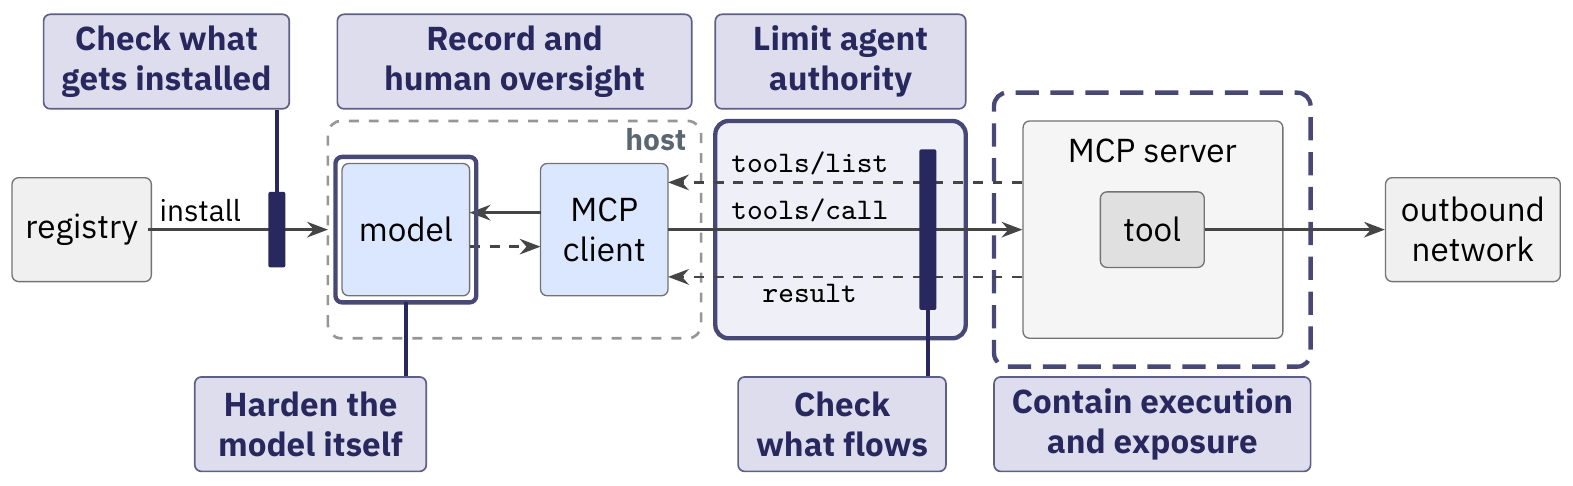
\includegraphics[width=0.85\textwidth]{figures/mitigations/mitigations-map-all.png}
  \caption{One tool call, from the installation of a tool to the outbound network, with the place
  where each mitigation family acts. The families are the course's grouping of ATLAS's
  mitigations.}
  \label{fig:mitigations-placement}
\end{figure*}

The base of the figure is an ordinary tool call over MCP (\cref{sec:mcp}). A tool is published in a
package registry (\cref{sec:threats-owasp}), such as the npm registry that distributed postmark-mcp,
and installed into the host.

The figure draws the model inside the host because the host makes every model call
(\cref{sec:mcp}). The model's tool calls reach the server only through the MCP client. The client
receives the tool definitions in reply to \demoref{tools/list}, sends \demoref{tools/call} and
receives the result from the MCP server. The server runs the tool, and the tool can open
connections that leave the machine, which the figure calls the outbound network.

Each family attaches to one part of this picture:
\bi
\item \textbf{Check what gets installed.} This family acts on the install arrow, before a model,
dataset, library or tool is trusted. Its members check an artifact's signature (Code Signing) or
its \textbf{cryptographic checksum}, a short value computed from a file's bytes that changes
whenever the file changes (Verify AI Artifacts). They also scan the artifact for known flaws and
unsafe calls (Vulnerability Scanning) \citep{mitre-atlas-2026}. Others test models and their
training data (Validate AI Model, Sanitize Training Data, Maintain AI Dataset Provenance). An
\textbf{AI bill of materials} is a list of every artifact used to build a system. Keeping one (AI
Bill of Materials) allows a rapid response when a vulnerability is reported in one of those
artifacts.
\item \textbf{Limit agent authority.} This family acts on the calls that cross from the client to
the server, by bounding what the agent may request. Its members set permissions for the agent, for
the user it acts for and for each shared tool. They block or confirm tool calls once untrusted data
is in the model's context, and they cap the tokens, iterations, tool calls, time and spending of a
run. \textbf{Least privilege} is the principle of granting a component only the rights its task
needs, and it underlies all the permissions mitigations. One member, AI Agent Authority Expansion
Controls, states that its control belongs outside the agent (\cref{sec:mitigations-enforcer}). The
family also holds three general limits on who may access a model and how often it may be queried.
\item \textbf{Check what flows.} This family acts on the messages themselves: the tool definitions,
the call and the result. A \textbf{guardrail} is a screen placed between users, tools and the model
that evaluates prompts, retrieved context, model outputs and tool requests before they are accepted
(Generative AI Guardrails). Input and Output Validation for AI Agent Components validates the
inputs and outputs of tools, outside the agent. Memory Hardening checks what an agent writes to its
persistent memory. The family's other members filter the inputs and outputs of predictive models,
which classify or score an input rather than generate content, or they detect generated media.
\item \textbf{Contain execution and exposure.} This family draws a boundary around the MCP server
and its tool. \textbf{Segmentation} isolates an agent's tools, data, identities and execution in
containers or virtual machines with restricted file and network access (Segmentation of AI Agent
Components). With segmentation in place, the arrow from the tool to the outbound network crosses a
boundary, where a connection can be refused. Restrict Library Loading also contains execution, by
stopping software from loading untrusted code. The family also limits exposure, meaning what an
adversary can learn about the system or reach in it. Encrypt Sensitive Information and three limits
on what an organization releases about its models serve this purpose.
\item \textbf{Record and human oversight.} This family watches the host, where the agent's steps
take place. \textbf{Telemetry} is the record that a system keeps of its own activity, here each
step of the agent, each data access and each tool call (AI Telemetry Logging). Human In-the-Loop
for AI Agent Actions requires a person to approve agent actions before they run. A \textbf{red
team} carries out recurring, authorized attack exercises against a system so that its flaws
are found and fixed (AI Red Team). AI Agent Scope Drift Detection, AI Honeypots and User Training
complete the family. A honeypot is a decoy, such as a fake AI service, agent or credential, that
legitimate users have no reason to use, so any use of it signals an adversary.
\item \textbf{Harden the model itself.} This family acts on the model. Generative AI Guidelines
give the model instructions and constraints, for example to treat retrieved content as untrusted.
Generative AI Model Alignment trains or fine-tunes the model toward safe behavior that stays within
its task. Both change the model, its training or its instructions so that it is harder to fool.
ATLAS maps both to AI Agent Tool Invocation, and they are the two mappings in this family's column
of \cref{tab:mitigations-coverage}. They are not in the tables that follow, and Lecture~6 discusses
them. Three measures for predictive models complete the family.
\ei

The families differ in what they act on. The \emph{Harden the model itself} family is the only one
that works by changing the model. The others act on something around it: an artifact before it
runs, the authority of a call, the content of messages, the place where a tool runs, or a record
and a person. The difference matters for enforcement, because a control that acts outside the model
still holds when an attack changes what the model does (\cref{sec:mitigations-enforcer}).

\subsection{Controls on agent authority}
\label{sec:mitigations-authority}

The mitigations of the \emph{Limit agent authority} family restrict an agent's identity, its
permissions, the authority it may acquire and the resources it may use \citep{mitre-atlas-2026}.
\Cref{tab:mitigations-authority,tab:mitigations-validation,tab:mitigations-oversight} list the
individual mitigations. Each table gives a mitigation's category, a condensed statement of what it
does, and the techniques of \cref{sec:attacks} that ATLAS maps it to, under these short names:
\bi
\item \textbf{Tool invocation} is AI Agent Tool Invocation, and \textbf{exfiltration} is
Exfiltration via AI Agent Tool Invocation.
\item \textbf{Context poisoning} is AI Agent Context Poisoning, and \textbf{resource consumption}
is Agentic Resource Consumption.
\item \textbf{Publishing a poisoned tool} is Publish Poisoned AI Artifacts: AI Agent Tools.
\item \textbf{Supply-chain compromise} is AI Supply Chain Compromise: AI Agent Tool, and
\textbf{user execution} is User Execution: Poisoned AI Agent Tool.
\ei
An asterisk marks a mapping to the parent technique. A sub-technique is one form of its parent, so
a countermeasure mapped to the parent applies to it as well.

The tables are a selection. They hold every mitigation that ATLAS maps to one of these techniques on
the technique's own entry, except Generative AI Guidelines and Generative AI Model Alignment, which
harden the model. They add Verify AI Artifacts and AI Bill of Materials, which reach the techniques
only through a parent technique. They also add AI Agent Authority Expansion Controls and AI Agent
Scope Drift Detection, which map to none of them. Other mitigations that are mapped only to a
parent technique are left out.

In \cref{tab:mitigations-authority}, notice that every permissions mitigation maps to the same two
techniques, tool invocation and exfiltration.

\begin{table*}[tb]
  \caption{Mitigations that restrict an agent's identity, permissions, authority and resource use,
  with the techniques of this lecture that ATLAS maps each one to.}
  \label{tab:mitigations-authority}
  \begin{adjustbox}{width=\linewidth}\begin{tabularx}{\linewidth}{L{0.24\linewidth}L{0.11\linewidth}XL{0.2\linewidth}}
    \toprule
    \textbf{Mitigation} & \textbf{Category} & \textbf{What it does} & \textbf{Lecture techniques it maps to} \\
    \midrule
    \textbf{Privileged AI Agent Permissions Configuration} & Technical (cyber) & Applies role-based,
    attribute-based and least-privilege controls to an agent that holds elevated rights &
    tool invocation, exfiltration \\
    \textbf{Single-User AI Agent Permissions Configuration} & Technical (cyber) & Gives an agent
    acting for one user no more rights than that user & tool invocation, exfiltration \\
    \textbf{AI Agent Tools Permissions Configuration} & Technical (cyber) & Gives shared tools the
    permissions and restrictions of the agent that calls them & tool invocation, exfiltration \\
    \textbf{Restrict AI Agent Tool Invocation on Untrusted Data} & Technical (AI) & Blocks or
    confirms tool calls once untrusted content has entered the model's context & tool invocation,
    exfiltration \\
    \textbf{Limit AI Workload Resource Consumption} & Technical (AI) & Bounds the tokens,
    iterations, tool calls, time and spending of one agent run & resource consumption \\
    \textbf{AI Agent Authority Expansion Controls} & Technical (AI) & Stops an agent from acquiring
    new permissions, tokens or targets during a run, enforced outside the agent & none of this
    lecture's techniques \\
    \bottomrule
  \end{tabularx}\end{adjustbox}
\end{table*}

The permissions mitigations apply least privilege to different holders of rights:
\bi
\item \textbf{A privileged agent.} Privileged AI Agent Permissions Configuration concerns an agent
granted rights above those of a normal user, or one that serves many users. It calls for
role-based and attribute-based access control, which grant rights according to the role a party
holds or according to attributes of the party, the resource and the request.
\item \textbf{An agent acting for one user.} Single-User AI Agent Permissions Configuration requires
that such an agent never hold a permission that the user would not be granted. The agent receives
its own identity, and it is decommissioned when its role ends. It works through \textbf{delegated
access}, acting with rights handed down from the party on whose behalf it works, here the user's
account.
\item \textbf{A shared tool.} AI Agent Tools Permissions Configuration concerns a tool that several
agents call. Through delegated access, the tool receives the permissions, identity and restrictions
of the agent that calls it.
\ei

These mitigations map to tool invocation and exfiltration because they bound what a steered agent
can do. An adversary who controls an agent's next action can invoke only the tools, and reach only
the resources, that the agent's permissions allow. Delegated access extends the bound to shared
tools, which cannot do for one agent what that agent could not do itself. Lecture~4's harness
applied the same principle to a single tool: the path check confined \demoref{edit} to the
workspace root.

Restrict AI Agent Tool Invocation on Untrusted Data responds to indirect prompt injection
(\cref{sec:threats-matrix}). Once text from a source outside the application's control has entered
the model's context, the mitigation blocks the automatic invocation of tools or asks the user to
confirm each call. The strictness depends on
the consequences of the action, and for high-consequence actions the mitigation recommends
confirmation every time. The mitigation does not try to recognize an injection. It reduces what an
injection can cause.

Limit AI Workload Resource Consumption bounds the tokens, iterations, retries, tool calls, time and
spending of one agent run. It counters Agentic Resource Consumption, in which an adversary coerces
an agent into costly calls, fan-outs or loops (\cref{sec:attacks}). One request can set off many
model calls and actions, so the limits apply to the whole run. The budget on model calls from
Lecture~2 and the resource limits on scripts from Lecture~4 are instances of this mitigation.

AI Agent Authority Expansion Controls stops an agent from acquiring new permissions, tokens or
targets during a run. The agent's maximum authority is granted before the run starts. Anything the
agent discovers during the run, such as a new resource, identity, service or target, stays outside
its scope until it is independently validated and added. ATLAS maps this mitigation to none of this
lecture's techniques. It matters here because it is one of the mitigations that say where a control
must sit (\cref{sec:mitigations-enforcer}).

\subsection{Validation and containment controls}
\label{sec:mitigations-validation}

These mitigations inspect what passes through a tool, a model or a memory, and they isolate where
code runs \citep{mitre-atlas-2026}. Input and Output Validation for AI Agent Components, Generative
AI Guardrails and Memory Hardening belong to the \emph{Check what flows} family, and Segmentation of
AI Agent Components belongs to the \emph{Contain execution and exposure} family. In
\cref{tab:mitigations-validation}, notice that validation and segmentation map to the same two
techniques as the permissions mitigations.

\begin{table*}[tb]
  \caption{Mitigations that inspect what passes through a tool, a model or a memory, and that
  isolate where code runs, with the techniques of this lecture that ATLAS maps each one to. An
  asterisk marks a mapping to the parent technique.}
  \label{tab:mitigations-validation}
  \begin{adjustbox}{width=\linewidth}\begin{tabularx}{\linewidth}{L{0.24\linewidth}L{0.11\linewidth}XL{0.2\linewidth}}
    \toprule
    \textbf{Mitigation} & \textbf{Category} & \textbf{What it does} & \textbf{Lecture techniques it maps to} \\
    \midrule
    \textbf{Input and Output Validation for AI Agent Components} & Technical (AI) & Validates the
    format and content of tool inputs and outputs, performed outside the agent & tool invocation,
    exfiltration \\
    \textbf{Generative AI Guardrails} & Technical (AI) & Screens prompts, retrieved context, outputs
    and tool requests between users, tools and the model & supply-chain compromise*, tool
    invocation \\
    \textbf{Memory Hardening} & Technical (AI) & Checks and constrains what is written to and read
    from an agent's persistent memory & context poisoning \\
    \textbf{Segmentation of AI Agent Components} & Technical (cyber) & Isolates agent tools, data,
    identities and execution in containers or virtual machines with restricted file and network
    access & tool invocation, exfiltration \\
    \bottomrule
  \end{tabularx}\end{adjustbox}
\end{table*}

Input and Output Validation for AI Agent Components checks the format and the content of what tools
receive and return. A format check includes schema validation. The MCP specification requires a
server to validate all tool inputs (\cref{sec:mcpcontract}), and checking the arguments against the
input schema is one way to meet that requirement. A content check looks
for sensitive information leaving in the data, and it removes injected instructions or unsafe code.
Exfiltration calls for content checks. The stolen data travels in the arguments of a call that is
well formed and authorized (\cref{sec:attacks}), so a check of the format alone lets it pass. The
mitigation adds that validation should be performed outside the agent, a requirement that
\cref{sec:mitigations-enforcer} examines.

Generative AI Guardrails puts the guardrails of \cref{sec:mitigations-placement} in the path of
every prompt, retrieved passage, model output and tool request. A guardrail can be a fixed rule,
such as an allowlist or a schema, or a model that classifies content. A guardrail differs from a
guideline of the \emph{Harden the model itself} family. A guideline asks the model to behave in a
certain way, whereas a guardrail checks what actually passes. ATLAS maps guardrails to tool
invocation, and through the parent technique to supply-chain compromise.

Memory Hardening checks and constrains what is written to and read from an agent's persistent
memory, the files or stored conversations that later sessions load. It counters context poisoning,
in which an instruction planted in memory fires in a later session as trusted input
(\cref{sec:attacks-memory}). Its controls include access control on memory operations, a record of
the source of every update, and rollback to a known good version. In the second attack on OpenClaw
(\cref{sec:openclaw-c2}), an instruction appended to the prompt file \demoref{HEARTBEAT.md} reached
every new conversation thread. ATLAS records the append as a change to the agent's configuration
\citep{atlas-cs0051-openclaw-c2}. It records the effect as AI Agent Context Poisoning, through the
Thread sub-technique. ATLAS maps Memory Hardening to AI Agent Context Poisoning and to its Memory
sub-technique, and it maps only AI Red Team to the Thread sub-technique.

Segmentation of AI Agent Components applies the sandbox of Lecture~4 (\cref{sec:attacks-escape}) to
every component of an agent. It maps to tool invocation and exfiltration: a tool whose network access is restricted can send data
only where its restrictions allow, whatever its arguments. ATLAS maps no mitigation to Escape to
Host, the technique that crosses this boundary (\cref{tab:mitigations-coverage}).

\subsection{Tool vetting, logging and human approval}
\label{sec:mitigations-oversight}

These mitigations vet what is installed, keep a record of what the agent does, and put a person in
the path of consequential actions (\cref{tab:mitigations-oversight}). Verify AI Artifacts,
Vulnerability Scanning and AI Bill of Materials belong to the \emph{Check what gets installed}
family, and the other mitigations in the table belong to the \emph{Record and human oversight}
family. In the table, notice that the vetting mitigations reach the supply-chain techniques mostly
through parent techniques, while the record and approval mitigations map to the tool call.

\begin{table*}[tb]
  \caption{Mitigations that vet what is installed, keep a record of what the agent does and put a
  person in the path of consequential actions, with the techniques of this lecture that ATLAS maps
  each one to. An asterisk marks a mapping to the parent technique.}
  \label{tab:mitigations-oversight}
  \begin{adjustbox}{width=\linewidth}\begin{tabularx}{\linewidth}{L{0.24\linewidth}L{0.11\linewidth}XL{0.2\linewidth}}
    \toprule
    \textbf{Mitigation} & \textbf{Category} & \textbf{What it does} & \textbf{Lecture techniques it maps to} \\
    \midrule
    \textbf{Verify AI Artifacts} & Technical (cyber) & Compares a cryptographic checksum to confirm
    an artifact was not modified & supply-chain compromise*, user execution* \\
    \textbf{Vulnerability Scanning} & Technical (cyber) & Scans model files, products and
    dependencies for unsafe calls and known flaws before use & publishing a poisoned tool, user
    execution* \\
    \textbf{AI Bill of Materials} & Policy & Lists every artifact used to build the system, which
    enables a rapid response to reported vulnerabilities & supply-chain compromise*, user
    execution* \\
    \textbf{AI Telemetry Logging} & Technical (cyber) & Records each step, data access, tool call
    and identity of an agent & tool invocation, exfiltration \\
    \textbf{Human In-the-Loop for AI Agent Actions} & Technical (AI) & Requires a person to approve
    agent actions before they run & tool invocation, exfiltration \\
    \textbf{AI Red Team} & Policy, technical (AI) and technical (cyber) & Runs recurring authorized
    attack exercises to find and fix flaws & supply-chain compromise, tool invocation, context
    poisoning, resource consumption \\
    \textbf{AI Agent Scope Drift Detection} & Technical (AI) & Watches whether an agent's planned
    actions still match its authorized objective, and can pause it if not & none of this lecture's
    techniques \\
    \bottomrule
  \end{tabularx}\end{adjustbox}
\end{table*}

Verify AI Artifacts compares an artifact's cryptographic checksum with the expected value
\citep{mitre-atlas-2026}. A match shows that the artifact has not been modified since it was
published. It cannot show that the published artifact is benign. In the rug pull of postmark-mcp
(\cref{sec:attacks}), the malicious version was itself the published version, so verifying its
checksum would only have confirmed the malicious code.

Vulnerability Scanning examines model files, products and dependencies for unsafe calls and known
flaws before they are used. A known flaw is one already reported, for example under a CVE
identifier (\cref{sec:inspector}). Scanning maps to the publication of a poisoned tool on that
technique's own entry, the single mapping in the \emph{Check what gets installed} column of
\cref{tab:mitigations-coverage}.

AI Bill of Materials is a policy: the organization keeps an AI bill of materials for each system.
Its value comes after a report. When a component is found to be vulnerable or malicious, the list
shows which systems include it, so that they can be found and repaired quickly. After postmark-mcp
was exposed, such a list would have shown which deployments had installed the malicious version.

AI Telemetry Logging records each step, data access, tool call and identity of an agent. The trace
that the course's harness writes, introduced in Lecture~2 as the log of a run's events, is
telemetry of this kind. A log prevents nothing by itself. It allows someone to detect an attack,
reconstruct what happened and respond.

Human In-the-Loop for AI Agent Actions requires a person to approve an agent's actions before they
run. It corresponds to consent in MCP: hosts must obtain the user's consent before invoking a tool,
and the protocol cannot enforce this requirement itself (\cref{sec:mcp-path}). It is also Lecture~2's
human-in-the-loop pattern, in which a run stops at points fixed at design time and waits for a
person to decide. Approvals cost time, so the mitigation scales them to the consequences of the
action. Minor, repetitive actions need little oversight, and actions with significant consequences
may need several approvers.

A person can refuse a harmful call only if the approval request shows the part of the call that
causes the harm. In the WhatsApp case (\cref{sec:attacks-exfiltration}), the confirmation dialog for a message
showed only its beginning, and the exfiltrated data lay out of view
\citep{beurerkellner2025whatsapp}. The user approved a call whose arguments were not shown in full.

AI Red Team maps to more of this lecture's techniques than any other mitigation: supply-chain
compromise, tool invocation, context poisoning and resource consumption. ATLAS advises the red team
to choose the adversary behaviors it tests from ATLAS's own tactics and techniques.

AI Agent Scope Drift Detection watches whether an agent's planned actions remain consistent with
its authorized objective, and it can pause the agent when they do not. Its signals include tool use
that does not fit the task and attempts to reach resources outside the agent's scope. ATLAS maps it
to none of this lecture's techniques.

\subsection{Where a control is enforced}
\label{sec:mitigations-enforcer}

ATLAS places some controls outside the agent, and it leaves unnamed the process that should
enforce any of them. Every mitigation says what to restrict or check. Permissions name what an
agent may access, validation names what to inspect, segmentation names what to isolate, and logging
names what to record.

Where a control sits determines whether the agent can get around it. AI Agent Authority Expansion
Controls and Input and Output Validation for AI Agent Components both state where their control must
sit: authority expansion controls ``should be implemented outside the AI agent'', and validation
``should be performed external to the AI agent'' \citep{mitre-atlas-2026}. A check that runs inside
the agent's own process shares that process and its permissions with the agent (\cref{sec:mcp-inside}). An
attacker who controls the agent, or who reaches its configuration, can then switch the check off or
route around it.

The authority expansion mitigation also rules out the model as the only enforcer. Authority
expansion controls ``should not rely solely on system prompts, model alignment, or the agent
recognizing that an action is out of scope''. A system prompt is text in the model's context, and
other text in the same context, such as an injected instruction (Lecture~4), can steer the model.
Alignment makes safe behavior more likely. It gives no guarantee for any particular input. A control
that depends on the model's behavior fails exactly when an attack succeeds in changing that
behavior.

No mitigation names the process that enforces it, and none names a feature of the operating-system
kernel or a hardware component. Some mitigations come close. AI Agent Authority Expansion Controls
lists kinds of mechanism, such as policy engines, target allowlists and approval gates. AI Agent
Tools Permissions Configuration says that its configurations may live in the MCP servers that
connect agents to tools, or in a tool's own configuration files. These name a kind of mechanism or a
place where a setting is written. They leave open which process must check the setting.

The harness, the operating-system kernel (\cref{sec:attacks-escape}) and the network are all
candidates for enforcing a rule outside the model:
\bi
\item \textbf{The harness.} A check in the program that runs the agent, such as the dispatcher of
Lecture~4, sees every tool call with its name and arguments. When the check runs in the agent's own
process, it shares that process's permissions, and an attacker who controls the process can switch
it off. Such a check is outside the model. It is still inside the agent, and the two quotations
above ask for these controls to sit outside the agent.
\item \textbf{The operating-system kernel.} The operating system confines a process in a sandbox and
checks every file that the process actually opens, whatever path string the tool was given. A read
that slips past the harness's path check, as reads through \demoref{search} did in Lecture~4, still
reaches only the files that the sandbox allows.
\item \textbf{The network.} A component on the network path can allow or refuse each connection
that a tool opens, such as the outbound connection in \cref{fig:mitigations-placement}.
\ei
Each place sees different events. The harness sees tool calls, the operating-system kernel sees the
file and process operations of a process, and the network sees connections. Which place enforces which rule is a
design decision that ATLAS leaves to the builder of the system. Lecture~6 takes up this decision,
starting with the two mitigations that put the rule in the model itself.

The case study that follows shows a real agent whose controls lived in its own configuration, and
what attackers did once they reached that configuration (\cref{sec:openclaw}).

\subsection*{Key points}
\bi
\item In ATLAS, a mitigation is a countermeasure mapped to the techniques it counters and labeled
as a policy, a technical control for AI or a technical control for cyber security, and release
2026.09 holds 40 of them.
\item In release 2026.09, ATLAS maps most mitigations of the lecture's techniques to the tool call
and none to tool poisoning, the rug pull, User Execution: Poisoned AI Agent Tool, Credentials from AI
Agent Configuration or Escape to Host, although controls on later steps can still limit these
attacks.
\item The six mitigation families are the course's grouping of ATLAS's mitigations, and each acts
at a different point of a tool call: on installation, on the agent's authority, on the messages,
around the tool's execution, by recording activity and asking a person to approve, or on the model.
\item The permissions mitigations apply least privilege to a privileged agent, to an agent acting
for one user and to shared tools, so that an adversary who steers the agent can do no more than the
agent is allowed to do.
\item A matching checksum shows only that an artifact is unchanged since publication, and an
approval protects the user only from what the approval request shows.
\item ATLAS states that authority controls and validation should sit outside the agent, and that
authority controls should not rely solely on system prompts, alignment or the agent's own judgment,
because a control inside the agent's process or behavior can be disabled or bypassed.
\item No ATLAS mitigation names the process that enforces it, so whether the harness, the
operating-system kernel or the network enforces a given rule remains a design decision.
\ei
